\documentclass[../thesis.tex]{subfiles}
\graphicspath{{../gfx/}{gfx/}}
\begin{document}

\pagestyle{plain}
\chapter{Badania}

Rozdział ten poświęcony jest opisowi przebiegu badań oraz obserwacjom poczynionym na wynikach tych badań. 

\section{Przebieg badań}

Badania przeprowadzono dwuetapowo. W pierwszym etapie pominięto fazę grupowania atrybutów ale uwzględniono fazę imputacji, usuwania i~skalowania. Pominięcie grupowania było związane z dużym narzutem czasowym spowodowanym bardzo dużą liczbą dodatkowych kombinacji, które grupowanie wnosi do procesu obliczeń. Po analizie wyników z pierwszej fazy wyłoniono najkorzystniejsze warianty rodzin algorytmów i~przystąpiono do etapu drugiego. W części tej użyto algorytmów grupowania dla tych rodzajów rodzin, które najlepiej wypadły w~fazie pierwszej.

\subsection{Faza pierwsza}

\subsubsection{Opis przebiegu badań}

Badania w~fazie pierwszej zostały przeprowadzone w~następujący sposób. Dla każdego rozważanego algorytmu klasyfikacji (naiwny klasyfikator bayesowski, drzewo decyzyjne, las losowy, maszyna wektorów nośnych) oraz każdej metody imputacji (wartością średniej, wartością mediany) obliczone zostały wyniki następujących rodzin algorytmów:

\begin{enumerate}
  \item Rodzina bez pozostałych etapów przetwarzania wstępnego
  \item Rodzina z usuwaniem wszystkich kombinacji atrybutów
  \item Rodzina ze skalowaniem wszystkich kombinacji atrybutów
  \item Rodzina z usuwaniem i~skalowaniem wszystkich kombinacji atrybutów
\end{enumerate}
Dla tak policzonych zbiorów ocen jakości klasyfikacji obliczono trzy rankingi:
\begin{enumerate}
  \item Wg wrażliwości
  \item Wg precyzji
  \item Wg metryki F1
\end{enumerate}
Rezultaty badań (kolejność rodzin w~rankingach, wzajemne relacje rodzin w~rankingach, wartości odpowiednich miar jakości klasyfikacji) poddano analizie.

\subsubsection{Analiza najlepszych rodzin w~rankingach}

Dla danych opisanych w~punkcie \ref{req:input} w~rankingu miar F1 najlepszą rodziną okazała się ta, która używała lasu losowego, skalowała wszystkie kombinacje atrybutów oraz imputowała brakujące wartości średnią. Rodzina ta zajęła jednocześnie drugie miejsce w~rankingu precyzji i~wrażliwości. Średnia wartość miary F1 wynosiła $0.8243$, a~odchylenie standardowe było równe $0.0368$. Rysunek \ref{results:histogram_f1_best} prezentuje histogram miar F1 dla tej rodziny.

\begin{figure}[h]
\centering
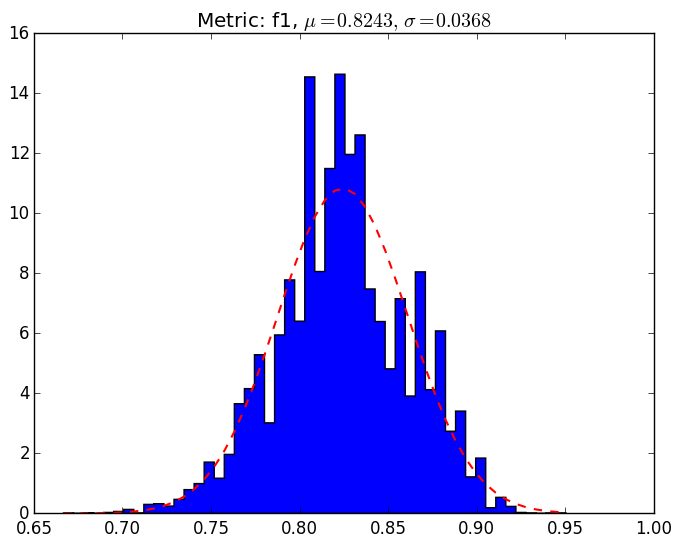
\includegraphics[width=0.9\textwidth]{10-f1.png}
\caption{Histogram miar oceny F1 dla najlepszej rodziny algorytmów w~rankingu F1. Linia przerywana to kontur zbliżonego rozkładu normalnego.}
\label{results:histogram_f1_best}
\end{figure}

Do ciekawych obserwacji można było dojść przyglądając się najlepszym dziesięciu rodzinom algorytmów. Aż sześć z nich używało klasyfikatora las losowy, a~pozostałe cztery drzewa decyzyjnego. Poza tym, połowa algorytmów imputowała braki medianą, a~druga połowa wartością średnią. 

W rankingu oceny precyzji klasyfikacji za najlepszą rodzinę została uznana ta, która używała lasu losowego, skalowała kombinacje atrybutów i~imputowała braki wartością mediany (średnia ocen $0.8499$, odchylenie $0.0313$). Co ciekawe, rodzina ta zajęła drugie miejsce w~rankingu miary F1. Histogram precyzji rodziny pokazano na rysunku \ref{results:histogram_p_best}.

\begin{figure}[h]
\centering
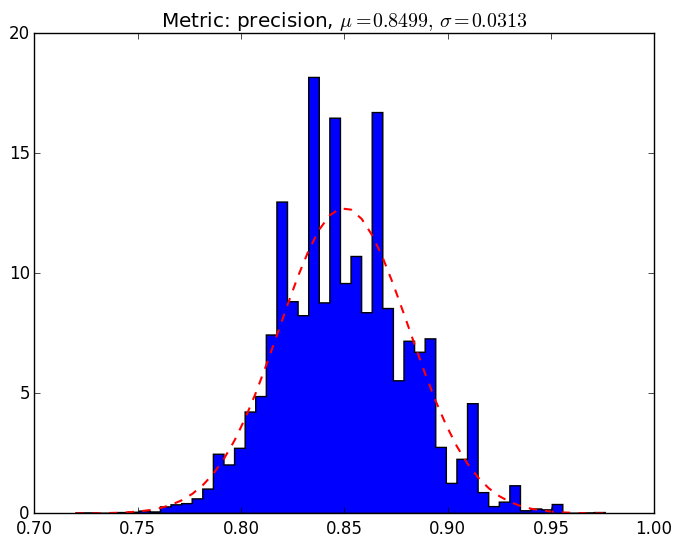
\includegraphics[width=0.9\textwidth]{13-precision.png}
\caption{Histogram precyzji dla najlepszej rodziny algorytmów w~rankingu precyzji. Linia przerywana to kontur zbliżonego rozkładu normalnego.}
\label{results:histogram_p_best}
\end{figure}

Podobnie jak w~przypadku rankingu miary F1, pierwsze 10 miejsc rankingu zostało zajętych przez rodziny używające klasyfikatora las losowy lub drzewo decyzyjne. Siedem na dziesięć rodzin użyło lasu losowego, trzy na dziesięć drzewa. Dodatkowo, tak jak poprzednio, połowa dziesięciu najlepszych rodzin imputowała medianą, a~druga połowa średnią.

Zwycięzcą rankingu wrażliwości została rodzina używająca maszyny wektorów nośnych jako klasyfikatora i~imputująca wartością średniej. Średnia wartość wrażliwości w~rodzinie wynosiła $0.9605$, a~odchylenie standardowe było równe $0.0773$. Histogram wrażliwości rodziny prezentuje ilustracja \ref{results:histogram_r_best}. 

\begin{figure}[h]
\centering
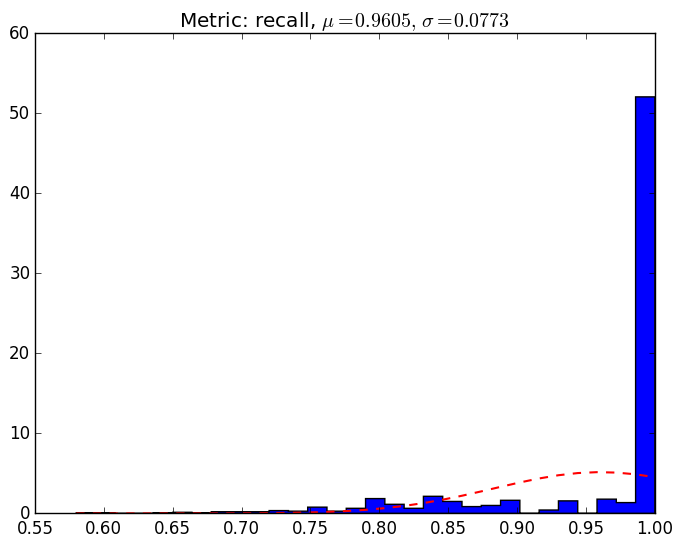
\includegraphics[width=0.9\textwidth]{68-recall.png}
\caption{Histogram wrażliwości dla najlepszej rodziny algorytmów w~rankingu wrażliwości. Linia przerywana to kontur zbliżonego rozkładu normalnego.}
\label{results:histogram_r_best}
\end{figure}

Cztery spośród dziesięciu najlepszych rodzin używało lasu losowego, trzy drzewa decyzyjnego, a~ostatnie trzy maszyny wektorów nośnych. Cztery na dziesięć rodzin imputowało medianą, sześć wartością średniej.

\subsubsection{Analiza kolejności rodzin w~rankingach}

Następna część analizy rankingów skupiła się na wpływie metod przetwarzania wstępnego na końcową pozycję rodziny w~rankingu. Dla danej metody klasyfikacji badane były pozycje rodzin używające różnych kombinacji etapów wstępnego przetwarzania. Pozycje rodzin w~rankingu przedstawia tabela \ref{results:table_rankings}.

\begin{table}[h]
\begin{center}
\begin{tabular}{ | l | l | p{100mm} | }
\hline
\rowcolor{lightgray} Ranking & Klasyfikator & Kolejność rodzin \\\hline

\multirow{4}{*}{F1} & Las losowy & pure, scale > remove+scale, remove \\\cline{2-3}
                    & Drzewo decyzyjne & scale > pure, remove+scale > remove\\\cline{2-3}
                    & Bayes & scale > remove+scale > remove > pure\\\cline{2-3}
                    & SVM & pure > scale > remove+scale > remove\\\hline
\multirow{4}{*}{Precyzja} & Las losowy & scale > pure > remove+scale > remove \\\cline{2-3}
                    & Drzewo decyzyjne & scale > remove+scale > pure > remove\\\cline{2-3}
                    & Bayes & scale > pure > remove+scale > remove\\\cline{2-3}
                    & SVM & remove+scale > scale, remove > pure\\\hline
\multirow{4}{*}{Wrażliwość} & Las losowy & pure, scale > remove+scale > remove \\\cline{2-3}
                    & Drzewo decyzyjne & scale > pure, remove+scale > remove\\\cline{2-3}
                    & Bayes & scale > remove+scale > remove > pure\\\cline{2-3}
                    & SVM & pure > scale > remove > remove+scale\\\hline

\end{tabular}
\caption{Kolejność w~rankingach rodzin używających różnych kombinacji etapów wstępnego przetwarzania. Oznaczenia: \emph{pure} - imputacja, \emph{remove} - imputacja z usuwaniem atrybutów, \emph{scale} - imputacja ze skalowaniem atrybutów, \emph{remove+scale} - imputacja z usuwaniem i~skalowaniem atrybutów.}
\label{results:table_rankings}
\end{center}
\end{table}

Dla wszystkich klasyfikatorów w~rankingu F1 skalowanie atrybutów działa lepiej niż skalowanie połączone z usuwaniem atrybutów. To zaś działa zawsze lepiej niż usuwanie kombinacji atrybutów. W rankingu precyzji rodziny usuwające i~skalujące atrybuty górują nad rodzinami, które tylko usuwają atrybuty. Spoglądając na wyniki wg rankingu wrażliwości, skalowanie atrybutów zawsze działa lepiej niż usuwanie lub usuwanie i~skalowanie atrybutów.

Niezależnie od tego, jaki rodzaj oceny chcemy maksymalizować, dla lasu losowego skalowanie zawsze sprawuje się lepiej niż skalowanie z usuwaniem bądź samo usuwanie atrybutów. Podobnie w~przypadku klasyfikatora, jakim jest drzew decyzyjne. W tym przypadku widać jednak jeszcze jedną regułę: skalowanie atrybutów działa lepiej niż prosty klasyfikator bez skalowania. Naiwny klasyfikator bayesowski, podobnie jak poprzednie, działa najlepiej gdy użyje się go ze skalowaniem atrybutów. Nie można niestety nic powiedzieć na temat generalnego wpływu etapów przetwarzania na jakość działania maszyny wektorów nośnych.

Powyższe wyniki jasno pokazują, że skalowanie atrybutów ma korzystny wpływ na jakość klasyfikacji dostępnych danych.

\subsubsection{Analiza całościowa}

Rozkłady ocen poszczególnych rodzin algorytmów były same w~sobie źródłem cennych informacji. Okazało się, że rodziny algorytmów używające naiwnego klasyfikatora bayesowskiego i~maszyny wektorów nośnych mają bardzo duże dysproporcje pomiędzy ocenami wrażliwości i~precyzji. Maszyna wektorów nośnych dawała bardzo wysokie wyniki wrażliwości (ok. 91\%), ale bardzo niskie wartości precyzji (ok. 56\%). Klasyfikator bayesowski odznaczał się natomiast bardzo niską wrażliwością (ok. 13\%). Tak niskie wartości ocen dyskwalifikują te dwa klasyfikatory. Przykładowe statystyki dla wybranych rodzin prezentuje tabela \ref{results:table_svm_bayes}.

\begin{table}[h]
\begin{center}
\begin{tabular}{ | l | l | l | }
\hline
\rowcolor{lightgray} Klasyfikator & Wrażliwość & Precyzja \\\hline

Bayes & $0.1355 \pm 0.0427$ & $0.7238 \pm 0.1130$\\\hline
Bayes & $0.1413 \pm 0.0402$ & $0.7626 \pm 0.1451$\\\hline
Bayes & $0.1318 \pm 0.1050$ & $0.7101 \pm 0.1743$\\\hline
SVM & $0.9205 \pm 0.0773$ & $0.5551 \pm 0.0899$\\\hline
SVM & $0.8902 \pm 0.1693$ & $0.5692 \pm 0.0918$\\\hline
SVM & $0.8904 \pm 0.1688$ & $0.5698 \pm 0.0922$\\\hline

\end{tabular}
\caption{Wartości średniej ocen i~odchylenia standardowego ocen dla wybranych rodzin algorytmów używających naiwnego klasyfikatora bayesowskiego (\emph{Bayes}) albo maszyny wektorów nośnych (\emph{SVM}).}
\label{results:table_svm_bayes}
\end{center}
\end{table}

\subsection{Faza druga}

\subsubsection{Opis przebiegu badań}

Analiza wyników z fazy pierwszej pokazała, że skalowanie atrybutów jest uniwersalną metodą polepszenia jakości klasyfikacji. W związku z tym, faza druga polegała na przeprowadzeniu etapów grupowania atrybutów dla uprzednio przeskalowanych atrybutów.

Dla każdej metody klasyfikacji (naiwny klasyfikator bayesowski, drzewo decyzyjne, las losowy, maszyna wektorów nośnych) oraz każdej metody imputacji obliczone zostały wyniki następujących rodzin:
\begin{enumerate}
  \item Jednokrotne grupowanie algorytmem \emph{K-Średnich} kombinacji przeskalowanych atrybutów o maksymalnej liczności równej 2.
  \item Jednokrotne grupowanie algorytmem \emph{Mean Shift} kombinacji przeskalowanych atrybutów o maksymalnej liczności równej 2.
\end{enumerate}
Rezultaty badań poddano analizie.

\subsubsection{Obserwacje}

Po potrzymaniu wyników okazało się, że działanie każdego algorytmu klasyfikacji wg każdego rankingu pogorszyło się po dodaniu etapu grupowania.

\section{Wnioski z badań}

Analiza wyników i~obserwacji prowadzi do następujących wniosków.

Mając na celu maksymalizację precyzji lub miary F1, najlepszym wyborem jest rodzina algorytmów używająca lasu losowego jako klasyfikatora oraz skalująca wartości wszystkich atrybutów. Metody te pozwalają osiągnąć wynik miary F1 rzędu 82\% oraz precyzji rzędu 85\%. Co ciekawe, wybór metody imputacji nie wpływa znacząco na ostateczną jakość predykcji.

Drugiem wnioskiem jest to, że rodziny używające lasu losowego lub drzewa decyzyjnego uzyskują najlepsze wyniki wszystkich rozpatrywanych miar jakości oceny (precyzji, wrażliwości, F1).

Kolejnym wnioskiem jest pozytywny wpływ skalowania atrybutów na działanie drzewa decyzyjnego i~naiwnego klasyfikatora bayesowskiego, bez względu na rozpatrywaną metrykę jakości oceny klasyfikacji.

W odróżnieniu od wyżej wymienionego skalowania, usuwanie atrybutów bardzo często prowadzi do pogorszenia jakości klasyfikacji. Co więcej, grupowanie atrybutów zawsze pogarsza ocenę.

Ostatecznie, naiwny klasyfikator bayesowski oraz maszyna wektorów nośnych, ze względu na niskie wartości wrażliwości i~predykcji, nie nadają się do klasyfikowania posiadanych danych medycznych.

\end{document}
